\documentclass[a4paper,12pt]{report}

\usepackage{alltt, fancyvrb, url}
\usepackage{graphicx}
\usepackage[utf8]{inputenc}
\usepackage{float}
\usepackage{hyperref}

\usepackage{amssymb}
\usepackage{amsmath}

% Questo commentalo se vuoi scrivere in inglese.
\usepackage[italian]{babel}

\usepackage[italian]{cleveref}
\bibliographystyle{plain}
\bibliography{references}

\linespread{1.28} % Imposta l'interlinea di x volte la dimensione del carattere

\title{Teoria dei numeri \\ applicata alla Crittografia}

\author{Giosuè Giocondo Mainardi\\ (n.0000933566)}
\date{\today}


\begin{document}

\maketitle

\tableofcontents
\chapter{Introduzione}
Nel vasto panorama della sicurezza informatica, la crittografia svolge un ruolo fondamentale nel garantire la confidenzialità, l'integrità e 
l'autenticità dei dati scambiati attraverso reti di comunicazione. All'interno di questa disciplina, la teoria dei numeri emerge come un 
pilastro imprescindibile, fornendo le fondamenta matematiche su cui molte tecniche crittografiche si basano.

Fino alla seconda metà del secolo scorso, si pensava che crittografia e matematica fossero due discipline distinte, 
addirittura \emph{G. H. Hardy}, noto matematico inglese di inizio '900, nel suo libro \emph{A Mathematician's Apology} (1940) affermava
che la matematica è una scienza neutra, pura e gentile, che non si schiera e non ha applicazioni dirette. 

Tuttavia, con l'avvento dell'informatica e della crittografia moderna, la teoria dei numeri ha assunto un ruolo di primaria importanza nello
sviluppo di algoritmi crittografici sicuri e affidabili. 
%
In particolare, algoritmi a chiave pubblica come RSA e DH, hanno dimostrato l'importanza della teoria dei numeri, attraverso l'uso della 
fattorizzazione in numeri primi e il logaritmo discreto.
%
La teoria dei numeri è un ramo della matematica che si occupa dello studio delle proprietà dei numeri interi, in particolare dei numeri primi e delle loro interazioni. 
Inoltre, tante volte in aritmetica i problemi sono semplici da porre ma difficili da risolvere, qualità che attirò l'attenzione già dai tempi 
dei greci e che torna utile quando si vuole nascondere un'informazione, come nel caso della crittografia.
In proposito, un'altra qualità importante è la casualità, la matematica è una scienza imprevedibile, ma sappiamo che la vera casualità è impossibile in aritmetica, citando \emph{Von Neumann}: 
\begin{quote}
	Anyone who considers arithmetical methods of producing random digits is, of course, in a state of sin.
\end{quote}

Nell'ambito di questa relazione, si esplorerà in dettaglio il legame stretto tra la teoria dei numeri e la crittografia, concentrandosi su concetti fondamentali come la fattorizzazione in numeri primi, il logaritmo discreto e le equazioni diofantee. Attraverso questa analisi approfondita, si intende fornire una panoramica esaustiva delle principali applicazioni della teoria dei numeri nel contesto della sicurezza informatica.
%
%
%
%
\chapter{Fondamenti della teoria dei numeri}
È importante fornire prima basi teoriche matematiche per comprendere il funzionamento degli algoritmi che andremo a trattare.

La teoria dei numeri è lo studio dei numeri interi, e delle loro proprietà. L'insieme dei numeri interi è $\mathbb{Z}$ e contiene tutti i numeri interi positivi e negativi, insieme allo zero.
\begin{quote}
	\centering
	..., -5, -4, -3, -2, -1, 0, 1, 2, 3, 4, 5, ...
\end{quote}
\section{Definizioni e concetti fondamentali della teoria dei numeri.}

\subsection*{Numero primo}
Un numero primo è un numero intero \( p > 1 \) che ha esattamente due divisori: 1 e \(p\) (se stesso).

\subsection*{Numero composto}
Un numero composto è un numero intero \( n > 1 \) che ha almeno un altro divisore, oltre 1 e \( n \) (se stesso).

\subsection*{Fattorizzazione}
La fattorizzazione è il processo di scomposizione di un numero intero \( n \) in un prodotto di numeri primi. Formalmente, data un numero intero \( n \), la fattorizzazione di \( n \) è data dalla rappresentazione \( n = p_1^{e_1} \cdot p_2^{e_2} \cdot \ldots \cdot p_k^{e_k} \), dove \( p_1, p_2, \ldots, p_k \) sono numeri primi distinti e \( e_1, e_2, \ldots, e_k \) sono esponenti positivi.

\subsection*{Concetti di divisibilità e criteri di divisibilità}

Un numero \(a\) è divisibile per un numero \(b\) se il resto della divisione di \(a\) per \(b\) è zero. In altre parole, se esiste un numero intero \(k\) tale che \(a = b \cdot k\), allora \(a\) è divisibile per \(b\).

\begin{itemize}
	\item \textbf{Criterio della divisibilità per 2}: Un numero è divisibile per 2 se il suo ultimo cifra è pari, cioè se termina con 0, 2, 4, 6 o 8.
	
	\item \textbf{Criterio della divisibilità per 3}: Un numero è divisibile per 3 se la somma delle sue cifre è divisibile per 3.
	
	\item \textbf{Criterio della divisibilità per 5}: Un numero è divisibile per 5 se termina con 0 o 5.
	
	\item \textbf{Criterio della divisibilità per 7}: Un numero è divisibile per 7 se il numero ottenuto sottraendo il doppio della cifra delle unità dal numero ottenuto togliendo la cifra delle unità è divisibile per 7.

	\item \textbf{Criterio della divisibilità per 11}: Un numero è divisibile per 11 se la differenza tra la somma delle cifre in posizione pari e la somma delle cifre in posizione dispari è divisibile per 11.

\end{itemize}

%\subsection*{Massimo comune divisore (MCD)}
%Il massimo comune divisore di due numeri interi \( a \) e \( b \), denotato come \( \mathbb{MCD}(a, b) \), è il più grande numero intero che divide entrambi \( a \) e \( b \) senza lasciare resto.

%\subsection*{Minimo comune multiplo (mcm)}
%Il minimo comune multiplo di due numeri interi \( a \) e \( b \), denotato come \( \mathrm{mcm}(a, b) \), è il più piccolo multiplo comune di \( a \) e \( b \).

\subsection*{Aritmetica Modulare}
L'aritmetica modulare è un ramo della teoria dei numeri che si occupa delle operazioni aritmetiche su numeri interi all'interno
di un insieme di resti modulo un numero fissato, noto come modulo. 

Inoltre, definisce un insieme di numeri interi con operazioni aritmetiche specifiche, che possono essere descritte come segue:

\subsubsection*{Definizione dell'insieme modulo}
Si sceglie un numero intero positivo \(m\), chiamato modulo, che determina l'insieme dei resti modulo \(m\). 
Questo insieme è denotato come \(\mathbb{Z}_m\) o \(\mathbb{Z}/m\), ed è composto da tutti i numeri interi che vanno da 0 a \(m-1\).

\subsubsection*{Congruenze}
Due numeri \( a \) e \( b \) sono congruenti modulo \( m \), denotato come \( a \equiv b \pmod{m} \), se \( a \) e \( b \) hanno lo stesso resto quando divisi per \( m \). Formalmente, \( a \equiv b \pmod{m} \) se e solo se \( m \) divide \( a - b \).

\subsubsection*{Definizione delle operazioni aritmetiche}
Sulle congruenze modulo \(m\), vengono definite le operazioni aritmetiche che rispettano le proprietà dell'insieme dei resti modulo \(m\):
\begin{itemize}
	\item \textbf{Addizione modulare}: \( (a + b) \mod m \)
	\item \textbf{Sottrazione modulare}: \( (a - b) \mod m \)
	\item \textbf{Moltiplicazione modulare}: \( (a \cdot b) \mod m \)
\end{itemize}

\subsubsection*{Proprietà dell'aritmetica modulare}
L'aritmetica modulare gode di alcune proprietà interessanti, tra cui la chiusura rispetto alle operazioni aritmetiche (cioè il risultato di un'operazione modulare è sempre un numero nell'insieme dei resti modulo \(m\)), l'associatività, la commutatività e la distributività.
%
%
%
\subsection*{Teorema cinese del resto}
Il teorema cinese del resto afferma che se \( m_1, m_2, \ldots, m_n \) sono interi positivi coprimi a coppie, e \( a_1, a_2, \ldots, a_n \) sono interi arbitrari, allora esiste un unico intero \( x \) che soddisfa il sistema di congruenze \( x \equiv a_1 \pmod{m_1}, x \equiv a_2 \pmod{m_2}, \ldots, x \equiv a_n \pmod{m_n} \).

\subsection*{Logaritmo discreto}
Il logaritmo discreto è definito come segue: date una base \( g \) e un modulo \( p \), il logaritmo discreto di \( b \) rispetto a \( g \) modulo \( p \), denotato come \( \log_g(b) \), è l'intero \( x \) tale che \( g^x \equiv b \pmod{p} \).

\subsection*{Curve ellittiche}
Le curve ellittiche sono insiemi di punti \( (x, y) \) che soddisfano un'equazione di forma cubica: \( y^2 = x^3 + ax + b \), dove \( a \) e \( b \) sono costanti. Le curve ellittiche hanno molte applicazioni in crittografia grazie alla loro proprietà di essere non solo additive ma anche moltiplicative.

\section{Sezione 1 Capitolo 2}

Contenuto.

\subsection*{Esempio}
Conseguentemente, GLaDOS è un ``observable'' per Output.

Qua esempio di immagine inserita sul posto.

\begin{figure}[h]
\centering{}
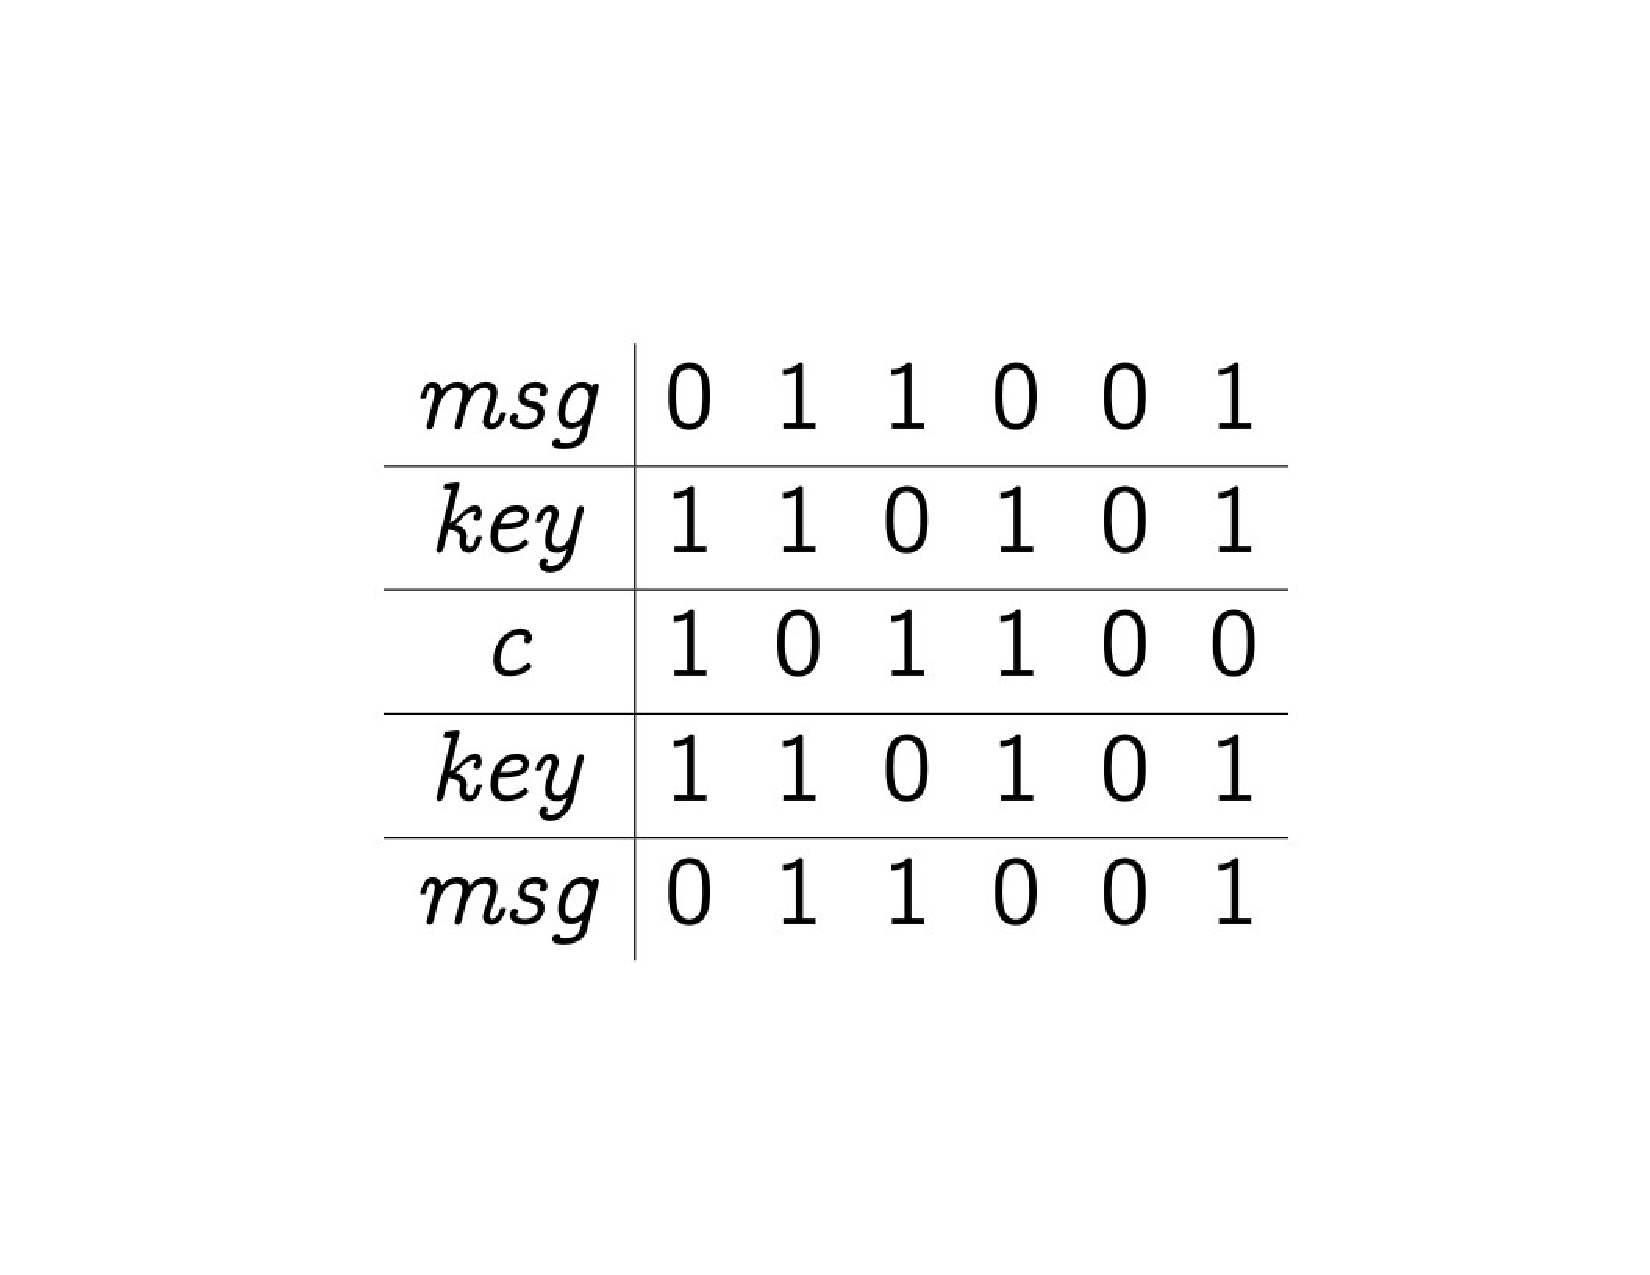
\includegraphics[width=\textwidth]{img/example_img.pdf}
\caption{L'interfaccia \texttt{GLaDOS}.}
\label{img:example}
\end{figure}

\section{Altra sezione}

\textbf{Sottotesto in grassetto}.

\subsection*{Esempio minimale}

\subsubsection{Sotto sotto sezione con paragrafi}

\paragraph{Paragrafo1} Contenuto.

\paragraph{Paragrafo Risposta 1} Contenuto \textit{paragrafo}, con riferimento immagine
\Cref{img:example}: e anche \texttt{Scrittura unicode}.

\chapter{Capitolo 3}
\section{Sezione}

Contenuto

\subsection{Esempio con sottosezioni e permalink}

\subsubsection{Utilizzo di \texttt{LoadingCache} dalla libreria Google Guava}

Permalink: \url{https://github.com/AlchemistSimulator/Alchemist/blob/d8a1799027d7d685569e15316a32e6394632ce71/alchemist-incarnation-protelis/src/main/java/it/unibo/alchemist/protelis/AlchemistExecutionContext.java#L141-L143}

\subsubsection{Utilizzo di \texttt{Stream} e lambda expressions}

Usate pervasivamente. Il seguente è un singolo esempio.
Permalink: \url{https://github.com/AlchemistSimulator/Alchemist/blob/d8a1799027d7d685569e15316a32e6394632ce71/alchemist-incarnation-protelis/src/main/java/it/unibo/alchemist/model/ProtelisIncarnation.java#L98-L120}

\subsubsection{Scrittura di metodo generico con parametri contravarianti}

Permalink: \url{https://github.com/AlchemistSimulator/Alchemist/blob/d8a1799027d7d685569e15316a32e6394632ce71/alchemist-incarnation-protelis/src/main/java/it/unibo/alchemist/protelis/AlchemistExecutionContext.java#L141-L143}

\chapter{Capitolo finale}

In quest'ultimo capitolo si tirano le somme del lavoro svolto e si delineano eventuali sviluppi
futuri.

\section{Sezione di commenti finali}

\textbf{È richiesta una sezione per ciascun membro del gruppo, obbligatoriamente}.

\appendix
\chapter{Capitolo appendice 1}

Contenuto.

\chapter{Capitolo appendice 2}

Contenuto.

\bibliographystyle{alpha}
\bibliography{report-template}

\end{document}
